
\subsection{Triple Integrals}
\FromC{\From Section 3.3 of \VCT.}
  
\BEN
% ~~~~~~~~~~~~~~~~~~~~~~~~~~~~~~~~~~~~~~~~~~~~~~~~~~~~~~~~~~~~~~~~~~~~~~~~~~~~~~~~~
\item % TETRAHEDRON
\Emph{Volume of a Tetrahedron} \\
The textbook points out that the triple integral 
\begin{align*}
  \iiint\limits_S f(x,y,z) dV
\end{align*}
for the special special case when $f(x,y,z) = 1$ for all points in $S$, gives the volume of $S$
\begin{align*}
  V(S) &= \iiint\limits_S dV.
\end{align*}
Consider again the tetrahedron that is bounded by the three coordinate planes in $\R^3$, and by the plane $z = 1 - x - \frac{y}{2}$. We derived an expression for the volume of this tetrahedron in a previous question using a double integral. Now set-up and find the volume of the tetrahedron using a triple integral.
% ~~~~~~~~~~~~~~~~~~~~~~~~~~~~~~~~~~~~~~~~~~~~~~~~~~~~~~~~~~~~~~~~~~~~~~~~~~~~~~~~~
\item % VOLUME OF AN ELLIPSOID
\textbf{Volume of an Ellipsoid}\\
Solve Question 10 from Section 3.5 of \VCT, which is the following: 
\begin{quotation}
\noindent
Show that the volume inside the ellipsoid $\frac{x^2}{a^2} + \frac{y^2}{b^2} + \frac{z^2}{c^2} = 1$ is $\frac{4\pi abc}{3}$ . (Hint: Use the
change of variables $x = au$, $y = bv$, $z = cw$, then consider Example 3.12.)
\end{quotation}
% ~~~~~~~~~~~~~~~~~~~~~~~~~~~~~~~~~~~~~~~~~~~~~~~~~~~~~~~~~~~~~~~~~~~~~~~~~~~~~~~~~
\item % MAXIMIZING A TRIPLE INTEGRAL
\textbf{Maximizing a Triple Integral}\\
Find the region $S$ for which the triple integral
\begin{align*}
  \iiint\limits_{S} \big(1 - 3x^2 - 2y^2 - 4z^2 \big)dV
\end{align*}
is a maximum. 

% ~~~~~~~~~~~~~~~~~~~~~~~~~~~~~~~~~~~~~~~~~~~~~~~~~~~~~~~~~~~~~~~~~~~~~~~~~~~~~~~~~
\EEN % END OF SUBSECTION
%
%% s~s~s~s~s~s~s~s~s~s~s~s~s~s~s~s~s~s~s~s~s~s~s~s~s~s~s~s~s~s~s~s~s~s~s~s~s~s~s~s~s~s~s~s
%% s~s~s~s~s~s~s~s~s~s~s~s~s~s~s~s~s~s~s~s~s~s~s~s~s~s~s~s~s~s~s~s~s~s~s~s~s~s~s~s~s~s~s~s
%\subsection{Change of Variables in Multiple Integrals}
%\FromC{\From Section 3.5 of \VCT.}
%\BEN
%% ~~~~~~~~~~~~~~~~~~~~~~~~~~~~~~~~~~~~~~~~~~~~~~~~~~~~~~~~~~~~~~~~~~~~~~~~~~~~~~~~~
%\item % GENERAL TRANSFORMATION
%\Emph{Linear Transformations} \\
%Under the linear transformation 
%\begin{align*}
%  x = c_1u + c_2v , \quad y =d_1u + d_2v, \quad d_1c_2 - d_2c_1 \ne 0,
%\end{align*}
%straight lines in the $uv$-plane are mapped to straight lines in the $xy$-plane. 
%\BEN
%\item $v=v_0$ is a horizontal line in the $uv$-plane. Determine the equation of this line in the $xy$-plane. 
%\item $x=x_0$ is a vertical line in the $xy$-plane. Determine the equation of this line in the $uv$-plane.
%\EEN
%% ~~~~~~~~~~~~~~~~~~~~~~~~~~~~~~~~~~~~~~~~~~~~~~~~~~~~~~~~~~~~~~~~~~~~~~~~~~~~~~~~~
%\item % STRAIGHTFORWARD CHANGE OF VARIABLES
%\Emph{Double Integral Over a Parallelogram} \\
%Use an appropriate transformation to evaluate the integral
%\begin{align*}
%  \iint\limits_R \big(x^2 - y^2\big) dxdy,
%\end{align*}
%where $R$ is the parallelogram bounded by 
%\begin{align*}
%  x+y = 0, \quad x+y = 1, \quad x-y=0, \quad x-y=1.
%\end{align*}
%
%% ~~~~~~~~~~~~~~~~~~~~~~~~~~~~~~~~~~~~~~~~~~~~~~~~~~~~~~~~~~~~~~~~~~~~~~~~~~~~~~~~~
%\item % SIMPLIFYING
%\Emph{Simplifying a Double Integral as a Product of Two Single Integrals} \\
%Show that, in the special case where the function $f(x,y)$ can be factored as the product $f(x,y) = g(x)h(y)$, the double integral 
%\begin{align*}
%   \iint\limits_{R} f(x,y) dA 
%\end{align*}
%can be written in the form
%\begin{align*}
%   \iint\limits_{R} g(x) h(y) dA 
%  & = \int_a^b g(x) dx \int_c^d h(y) dy  .
%\end{align*}
%where $R$ is the rectangular region $R=\{(x,y) | a \le x \le b, c\le y \le d\}$. 
%This result can be helpful in simplifying certain multiple integrals. 
%
%% ~~~~~~~~~~~~~~~~~~~~~~~~~~~~~~~~~~~~~~~~~~~~~~~~~~~~~~~~~~~~~~~~~~~~~~~~~~~~~~~~~
%\item % CHANGE OF VARIABLES TWICE
%\Emph{Triple Integral Bounded by an Ellipse} \\
%Use the transformation $x = 3u, y = 2v$ to evaluate the double integral
%\begin{align*}
%  \iint\limits_E x^2 \ dxdy,
%\end{align*}
%where $E$ is region bounded by the ellipse $4x^2 + 9y^2 = 36$. \textit{Hint: you may also want to use polar coordinates to solve this problem}.
%% ~~~~~~~~~~~~~~~~~~~~~~~~~~~~~~~~~~~~~~~~~~~~~~~~~~~~~~~~~~~~~~~~~~~~~~~~~~~~~~~~~
%\item % SIMPLE CYLINDRICAL WITH CONE
%Evaluate the integral
%\begin{align*}
%  \iiint\limits_S y^2dV,
%\end{align*}
%where $S$ is the solid that lies inside the cylinder $x^2+y^2 = 1$, above the plane $z=0$ and below the cone $z^2 = 9x^2 + 9y^2$. 
%% ~~~~~~~~~~~~~~~~~~~~~~~~~~~~~~~~~~~~~~~~~~~~~~~~~~~~~~~~~~~~~~~~~~~~~~~~~~~~~~~~~
%\item % TRIPLE INTEGRAL IN CYLINDRICAL COORDINATES
%\Emph{Triple Integral In Cylindrical Coordinates} \\
%Evaluate the integral
%\begin{align*}
%  \iiint\limits_V dV,
%\end{align*}
%using cylindrical coordinates, where $V$ is the region bounded by
%\begin{align*}
%  0 \le\ &x \le 2 \\
%  0 \le\ &y \le \sqrt{4 - x^2}\\
%  0 \le\ &z \le \sqrt{4 - (x^2+ y^2)}
%\end{align*} 
%% ~~~~~~~~~~~~~~~~~~~~~~~~~~~~~~~~~~~~~~~~~~~~~~~~~~~~~~~~~~~~~~~~~~~~~~~~~~~~~~~~~
%\item % TRIPLE INTEGRAL IN SPHERICAL COORDINATES
%\Emph{Triple Integral In Spherical Coordinates} \\
%The integral
%\begin{align*}
%  \mathop{\int_0^{\pi/4} \!\! \int_{0}^{\pi/2} \!\! \int_0^1 } ( \rho^2 \sin\phi ) \ d\rho\  d\phi\  d\theta
%\end{align*}
%represents the volume of a solid. Describe the shape of the solid, and find its volume. \\\rednote{Textbook doesn't do a great job of integrals in cylindrical and spherical}
%% ~~~~~~~~~~~~~~~~~~~~~~~~~~~~~~~~~~~~~~~~~~~~~~~~~~~~~~~~~~~~~~~~~~~~~~~~~~~~~~~~~
%\EEN % END OF SUBSECTION 
%% s~s~s~s~s~s~s~s~s~s~s~s~s~s~s~s~s~s~s~s~s~s~s~s~s~s~s~s~s~s~s~s~s~s~s~s~s~s~s~s~s~s~s~s
%% s~s~s~s~s~s~s~s~s~s~s~s~s~s~s~s~s~s~s~s~s~s~s~s~s~s~s~s~s~s~s~s~s~s~s~s~s~s~s~s~s~s~s~s
%\subsection{Application: Center of Mass}
%\FromC{\From Section 3.6 of \VCT.}
%\BEN
%% ~~~~~~~~~~~~~~~~~~~~~~~~~~~~~~~~~~~~~~~~~~~~~~~~~~~~~~~~~~~~~~~~~~~~~~~~~~~~~~~~~
%\item % CENTER OF MASS OF 2D TRIANGULAR PLATE
%\Emph{Center of Mass of a 2D Triangular Plate} \\
%A two-dimensional plate has density $\delta(x,y) = xy$, and occupies a triangular region whose vertices are located at the points (0,0), (1,2), and (1,4). Find the $x$-coordinate and the $y$-coordinate of the center of mass of the triangular plate. 
%% ~~~~~~~~~~~~~~~~~~~~~~~~~~~~~~~~~~~~~~~~~~~~~~~~~~~~~~~~~~~~~~~~~~~~~~~~~~~~~~~~~
%\item % CENTER OF MASS OF 2D RADIAL DENSITY FUNCTION
%\Emph{Center of Mass of a 2D Plate, Radial Density Function} \\
%A 2D semi-circular plate of mass $M$ is bounded by 
%\begin{align*}
%  -a \le x \le a, \quad 0 \le y \le \sqrt{a^2 - x^2}, \quad a > 0.
%\end{align*}
%The density of the plate at a point $(x,y)$, is equal to the shortest distance, $L$, between that point and the upper edge of the plate, as shown in Figure \ref{FigCircPlate}. 
%\BEN
%\item Set up an integral that represents the $x$-coordinate of the center of mass of the plate, $\bar{x}$. 
%\item Set up an integral that represents the $y$-coordinate of the center of mass of the plate, $\bar{y}$. 
%\item Determine the $x$-coordinate of the center of mass of the plate, without performing any integration. Briefly describe how you found your answer. 
%\EEN
%You do not need to perform any integration for this question. Note also that $L$ is a function of $x$ and $y$. 
%\begin{figure}[H]
%  \vspace{-1pt}
%  \begin{center}
%    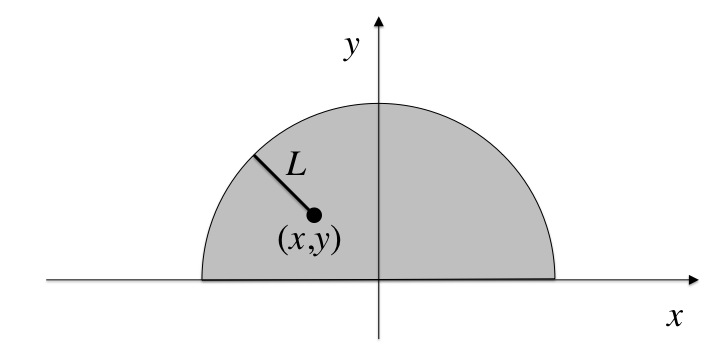
\includegraphics[width=0.65\textwidth]{ImgRadialCenterOfMass.jpg}
%  \end{center}
% \begin{quote} \caption{\label{FigCircPlate}\small{The density of the plate at $(x,y)$ is equal to $L$.}}\end{quote}
%\end{figure}
%% ~~~~~~~~~~~~~~~~~~~~~~~~~~~~~~~~~~~~~~~~~~~~~~~~~~~~~~~~~~~~~~~~~~~~~~~~~~~~~~~~~
%\item % MOMENTS OF A CYLINDER
%\Emph{Center of Mass of a 2D Plate, Radial Density Function} \\
%
%% ~~~~~~~~~~~~~~~~~~~~~~~~~~~~~~~~~~~~~~~~~~~~~~~~~~~~~~~~~~~~~~~~~~~~~~~~~~~~~~~~~
%\item % EVEN AND ODD
%\rednote{I'll push this question to a midterm or final exam}\\
%Determine the value of
%\begin{align*}
%  \mathop{\int_0^{\pi} \!\! \int_{-1}^1} x^4e^{x^2 + y^2}\sin(y) dydx.
%\end{align*}
%Do not use integration by parts.
%% ~~~~~~~~~~~~~~~~~~~~~~~~~~~~~~~~~~~~~~~~~~~~~~~~~~~~~~~~~~~~~~~~~~~~~~~~~~~~~~~~~
%
%
%% ~~~~~~~~~~~~~~~~~~~~~~~~~~~~~~~~~~~~~~~~~~~~~~~~~~~~~~~~~~~~~~~~~~~~~~~~~~~~~~~~~
%\item % CHANGING ORDER OF INTEGRATION
%\rednote{This is a good midterm question. I'll move it later.}\\
%\textbf{Changing the Order of Integration}\\
%The volume, $V$, of the solid bounded by
%\begin{align*}
%  z=0, \quad x=y^2, \quad x+z=1
%\end{align*}
%can be found using the triple integral 
%\begin{align*}
%  V = \mathop{\int_{0}^{1} \!\! \int_{-\sqrt{x}}^{\sqrt{x}} \! \int_0^{1-x} } dz\ dy\ dx = \frac{8}{15}.
%\end{align*}
%By simply changing the order of integration, we can find five other ways of expressing the volume of the solid. Find three of them. 
%
%Note that for this question, you do not need to perform any integration. Simply set up three other triple integrals that represent the volume of the solid.
%\textit{Hint: you may however want to check that your integrals represent the same volume with WolframAlpha}.
%
%\EEN % END OF SUBSECTION 
%
%
%
%
%
